\documentclass[9pt,a4paper]{report}
\usepackage{mwe}
\usepackage{listings}
\usepackage{amsmath}
\usepackage{graphicx}
\usepackage{subfig}
\usepackage{float}
\usepackage{xcolor}
\usepackage{multirow}
\usepackage{hyperref}
\usepackage{fancyhdr}
\usepackage{sectsty}
\usepackage[dvipsnames]{xcolor}
\usepackage{soul}
\usepackage[compact]{titlesec}
\usepackage{float}
\usepackage[left=0.5cm,right=0.5cm,top=0.5cm,bottom=0.5cm]{geometry}
\graphicspath{}

\newcommand*{\nchapter}[1]{%
	\chapter*{#1}%
	\addcontentsline{toc}{chapter}{#1}
	\vspace{-14mm}}
\newcommand*{\nsection}[1]{%
	\section*{#1}%
	\addcontentsline{toc}{section}{#1}}
\newcommand*{\nsubsection}[1]{%
	\subsection*{#1}%
	\addcontentsline{toc}{subsection}{#1}}
\newcommand*{\nsubsubsection}[1]{%
	\subsubsection*{#1}%
	\addcontentsline{toc}{subsubsection}{#1}}

\chaptertitlefont{\large}
\sectionfont{\normalsize}
\fontsize{9}{11}\selectfont
\begin{document}
	\begin{titlepage}
		\centering
		\vspace*{1.5in}
		
\includegraphics[width=0.15\textwidth]{W-Logo_Purple_RGB}\par\vspace{1cm}
		{\LARGE \textsc{University of Washington}\par}
		\vspace{1cm}
		{\Large \textsc{BEE331 Lab 2.1}\par}
		\vspace{1.5cm}
		{\huge\bfseries \par}
		\vspace{2cm}
		{\Large\itshape 2301991\hspace{55pt}2130474\par}
		{\Large\itshape Jason Truong\hspace{31pt}Henry Haight\par}
		\vfill
		supervised by\par
		Prof.~Joseph \textsc{Decuir}
		\date{2024\\ January}
		\vfill
		% Bottom of the page
		{\large \today\par}
		\vspace*{1.5in}
	\end{titlepage}
	
	\newpage
	\nchapter{Addendum Pages}
	\begin{figure}[hp!]
		\centering
		\caption{Jason Truong Addendum}
		%\subfloat[\centering Lab Design   Calculations]{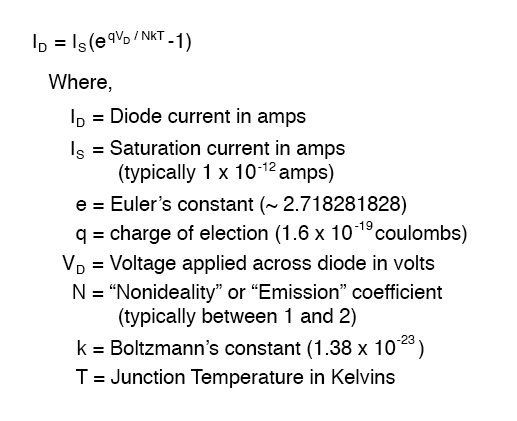
\includegraphics[width=17cm]{Theoretical Calculation of Ideal Diode}}
	\end{figure}
	\newpage
	\nsection{Bibliography}
	\textbf{Cited:}\\
	\begin{itemize}
		\item Lab 1 Manual
		\item Sedra, Adel, and Kenneth Smith. Microelectronic Circuits. S.L., Oxford Univ Press Us, 2019.
	\end{itemize}
	\begin{figure}[!h]
		\subfloat[Penance.]{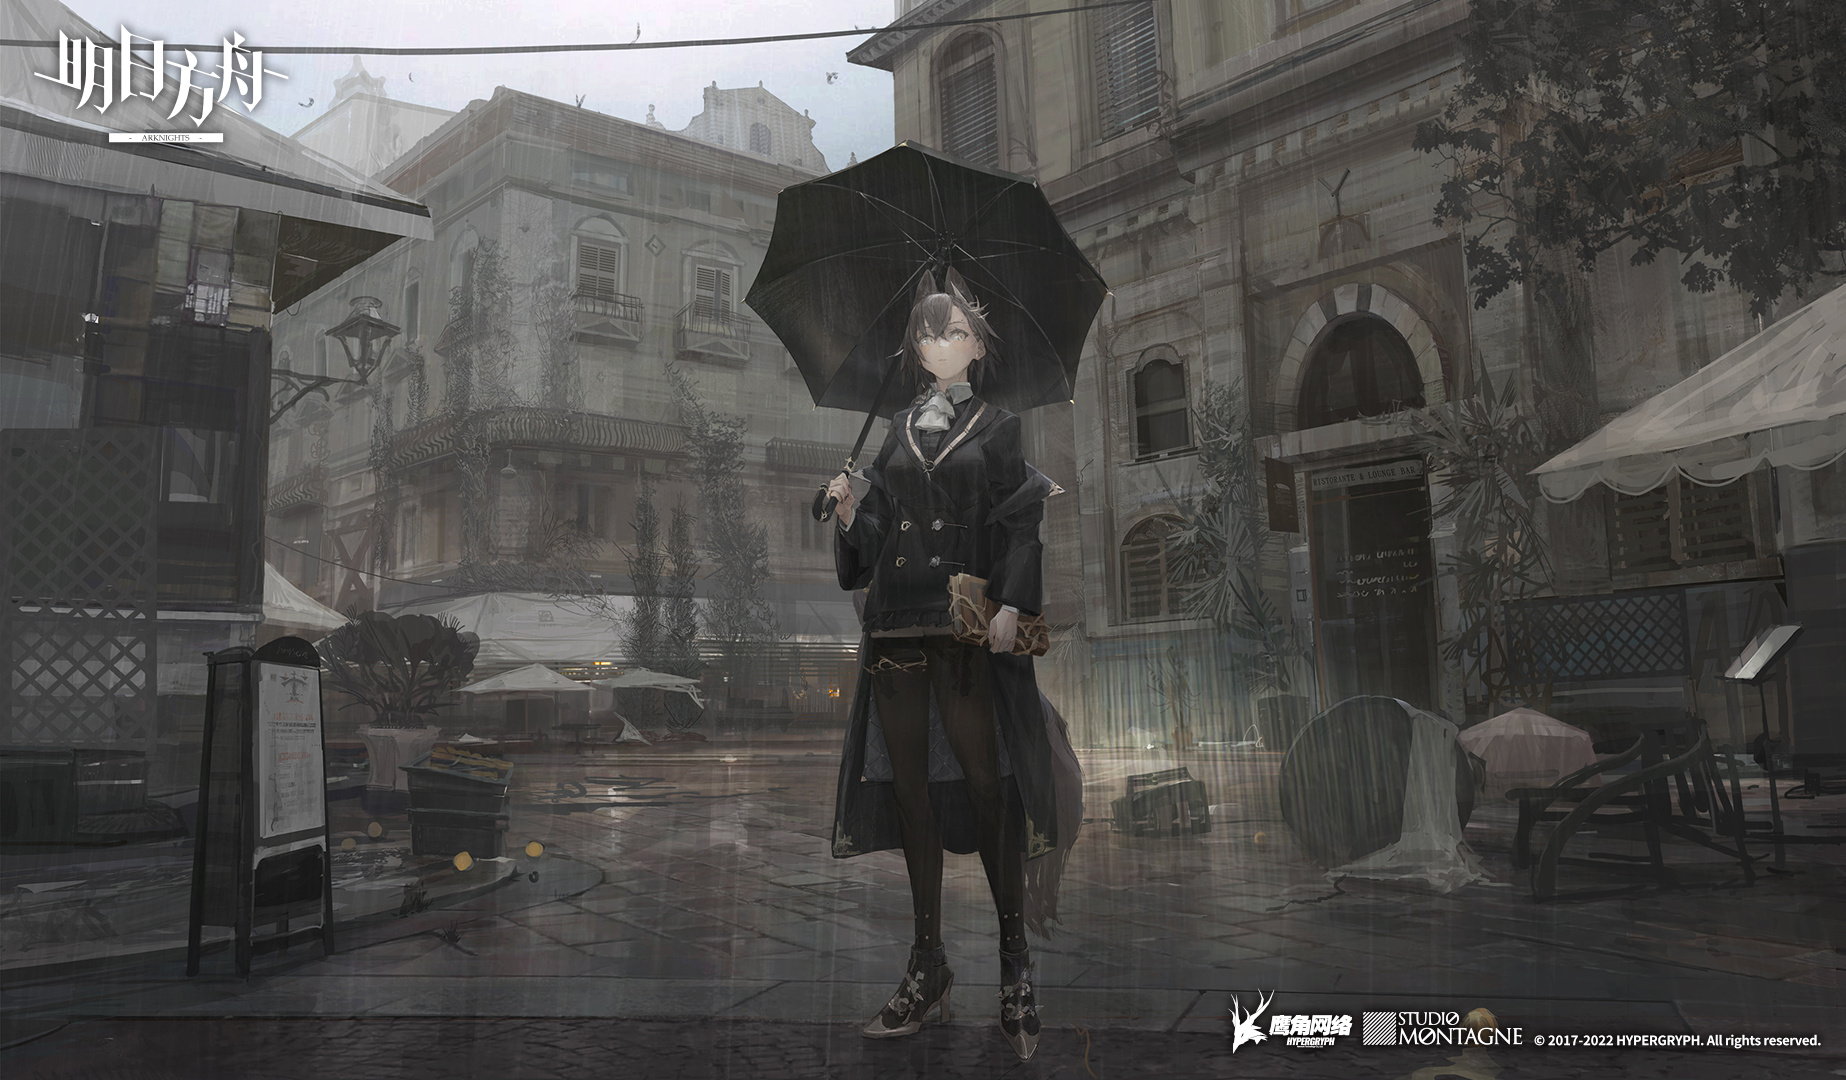
\includegraphics[width=\linewidth]{2053eee52228f604772553bcfd001b6a2d3d0be0}}
	\end{figure}
\end{document}